\documentclass[border=5pt]{standalone}
\usepackage{tikz,graphicx,amsmath,amssymb,xcolor}\usepackage{fontspec,xeCJK}\setmainfont{Helvetica}\setCJKmainfont{PingFang SC}
\usetikzlibrary{arrows.meta}
\definecolor{ink}{HTML}{203D46}\definecolor{teal}{HTML}{277A80}\definecolor{pale}{HTML}{EFF6F5}\definecolor{warm}{HTML}{F6ECDD}
\begin{document}\begin{tikzpicture}[x=1mm,y=1mm,font=\fontsize{11}{14}\selectfont,text=ink]
\path[use as bounding box] (0,0) rectangle (105,260);
\node[anchor=north west,font=\bfseries\fontsize{16}{19}\selectfont] at (3,258) {DINO：一张图走完整条链};
\node[anchor=north west,text width=98mm,font=\fontsize{10}{13}\selectfont] at (3,248) {训练：A 分别送学生/教师，$B\to C$ 对齐；D 更新教师与中心。使用：骨干进入 E，训练头退场。};
\fill[pale,rounded corners=2mm] (1,191) rectangle (104,232);
\node[anchor=north west,text=teal,font=\bfseries\fontsize{12}{15}\selectfont] at (4,230) {A 同一图，换几个看法 · §3.1};
\node[anchor=north west,text width=66mm,inner sep=0] at (4,222) {2 个 $224^2$ 全局裁剪\\6 个 $96^2$ 局部裁剪\\学生看全部，教师只看全局\\输入来自同一张图};
\node[anchor=center,inner sep=0] at (88,208) {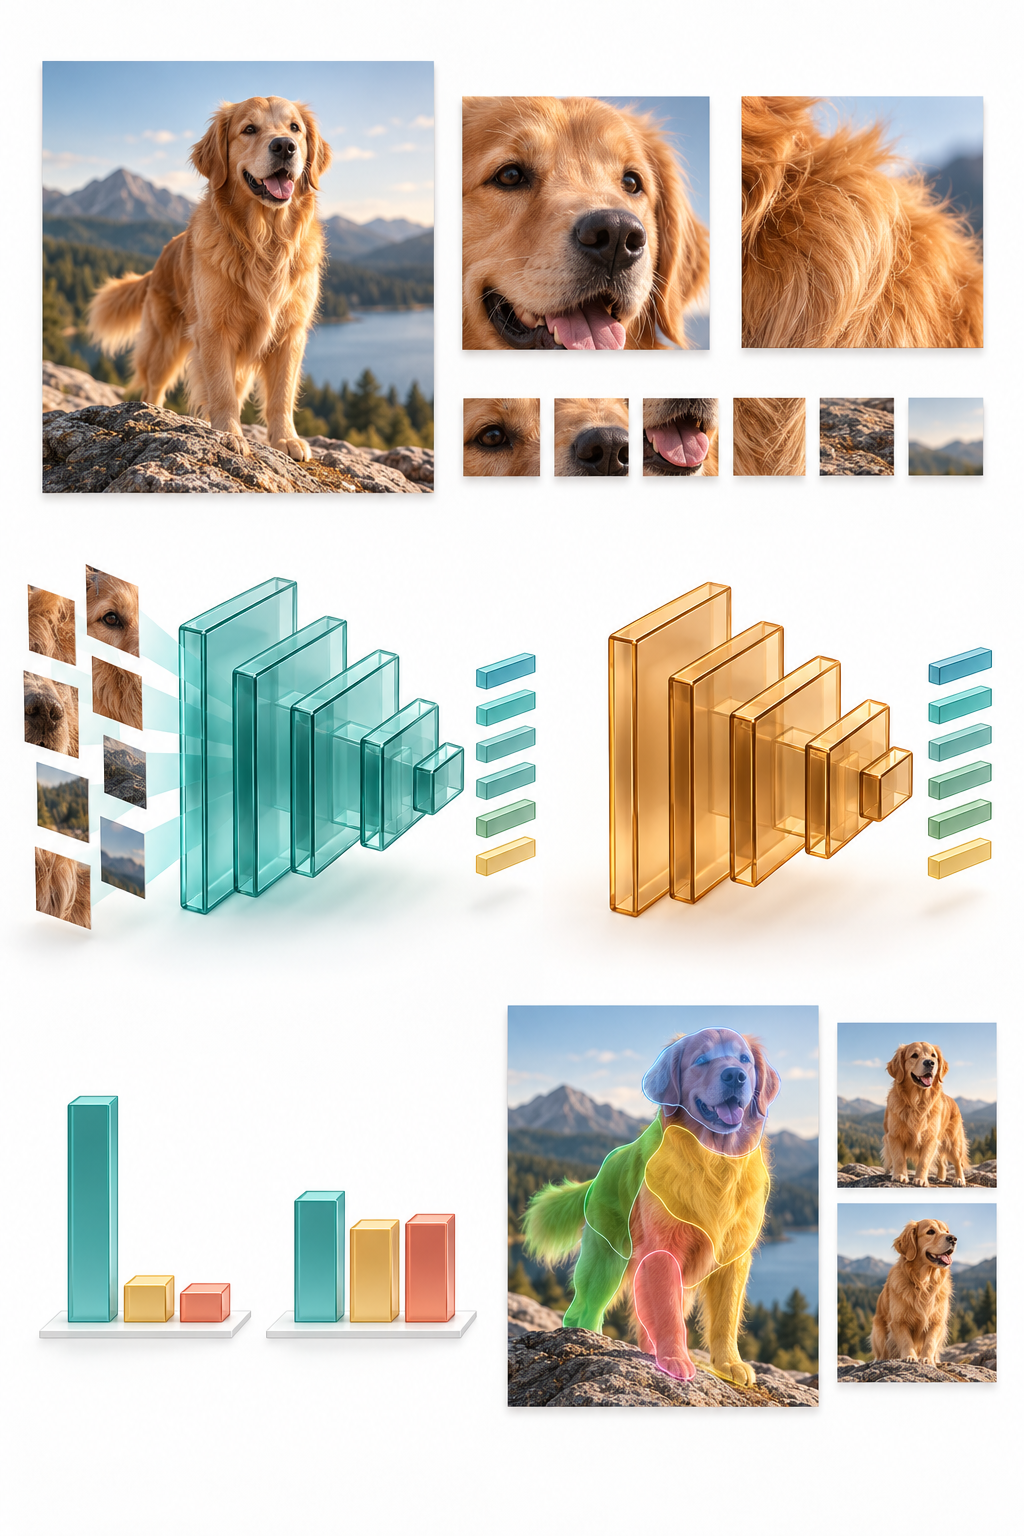
\includegraphics[width=26mm,height=31mm,keepaspectratio,viewport=35 1016 1000 1506,clip]{dino-imagegen-draft.png}};
\draw[-{Latex[length=2mm]},teal,line width=.7pt] (52.5,190.5) -- (52.5,187);
\fill[pale,rounded corners=2mm] (1,145) rectangle (104,186);
\node[anchor=north west,text=teal,font=\bfseries\fontsize{12}{15}\selectfont] at (4,184) {B 两路网络 · §3.1–3.2};
\node[anchor=north west,text width=66mm,inner sep=0] at (4,176) {同结构，不同参数\\ViT-S/16：$197\times384$\\CLS $\rightarrow$ MLP $\rightarrow256$\\归一化投影到 $K=65536$};
\node[anchor=center,inner sep=0] at (88,162) {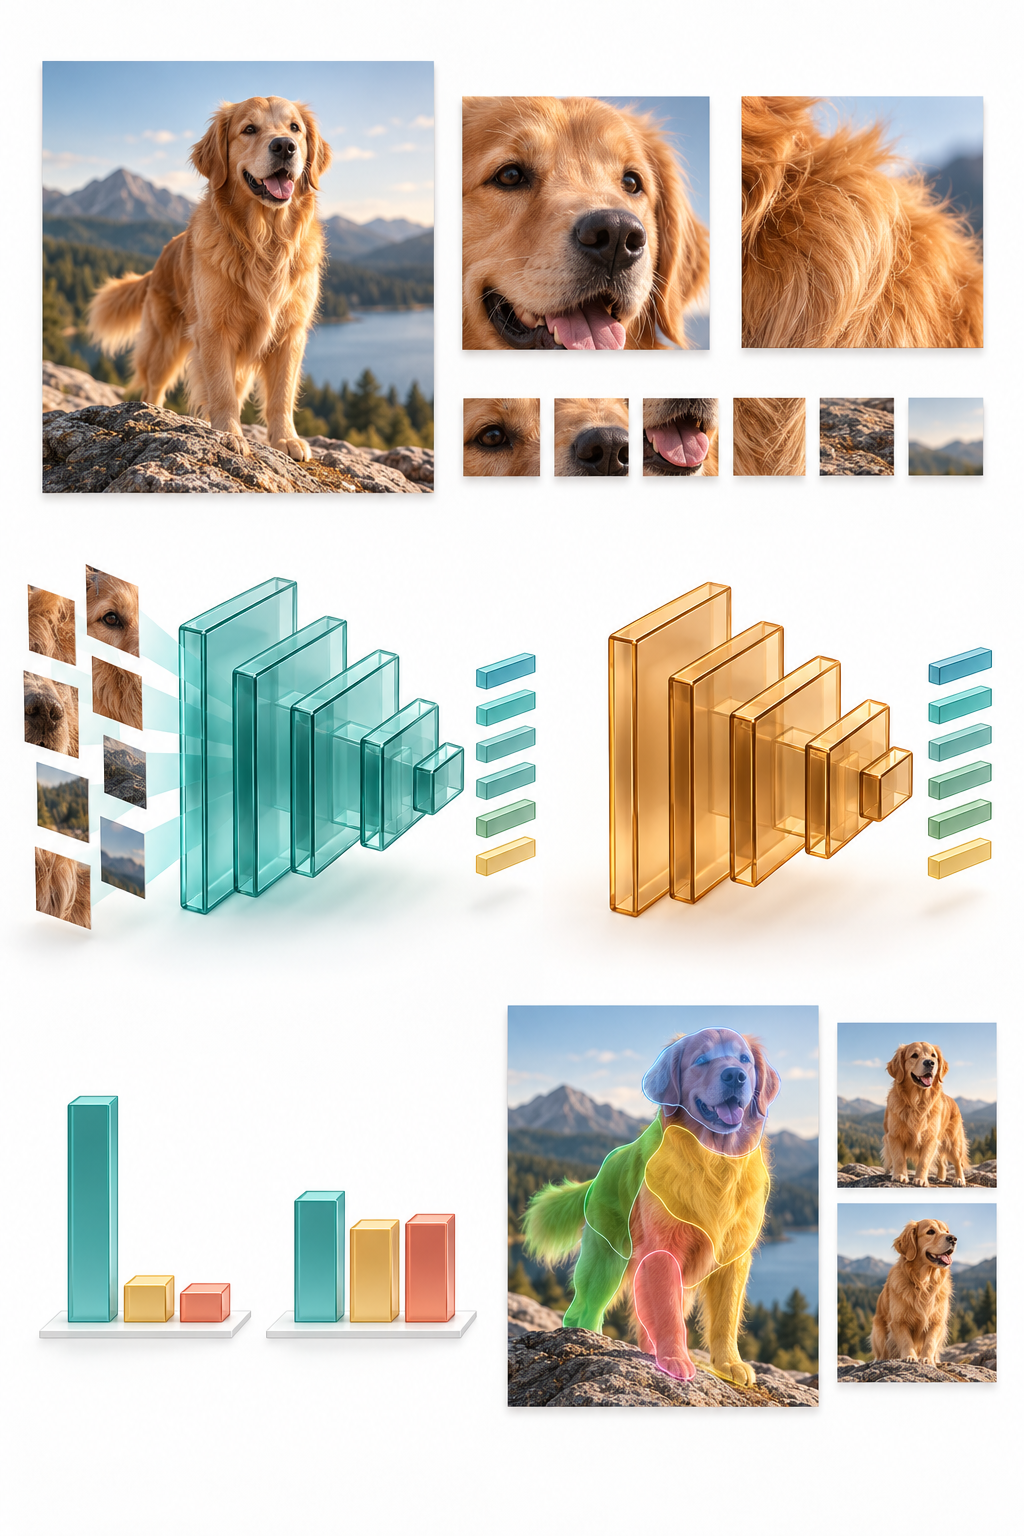
\includegraphics[width=26mm,height=31mm,keepaspectratio,viewport=20 536 510 1046,clip]{dino-imagegen-draft.png}};
\draw[-{Latex[length=2mm]},teal,line width=.7pt] (52.5,144.5) -- (52.5,141);
\fill[pale,rounded corners=2mm] (1,99) rectangle (104,140);
\node[anchor=north west,text=teal,font=\bfseries\fontsize{12}{15}\selectfont] at (4,138) {C 对齐概率分布 · §3.1};
\node[anchor=north west,text width=66mm,inner sep=0] at (4,130) {教师：减中心 + 低温 softmax\\学生：softmax\\跨视图交叉熵，只更新学生\\教师分布停止梯度};
\node[anchor=center,inner sep=0] at (88,116) {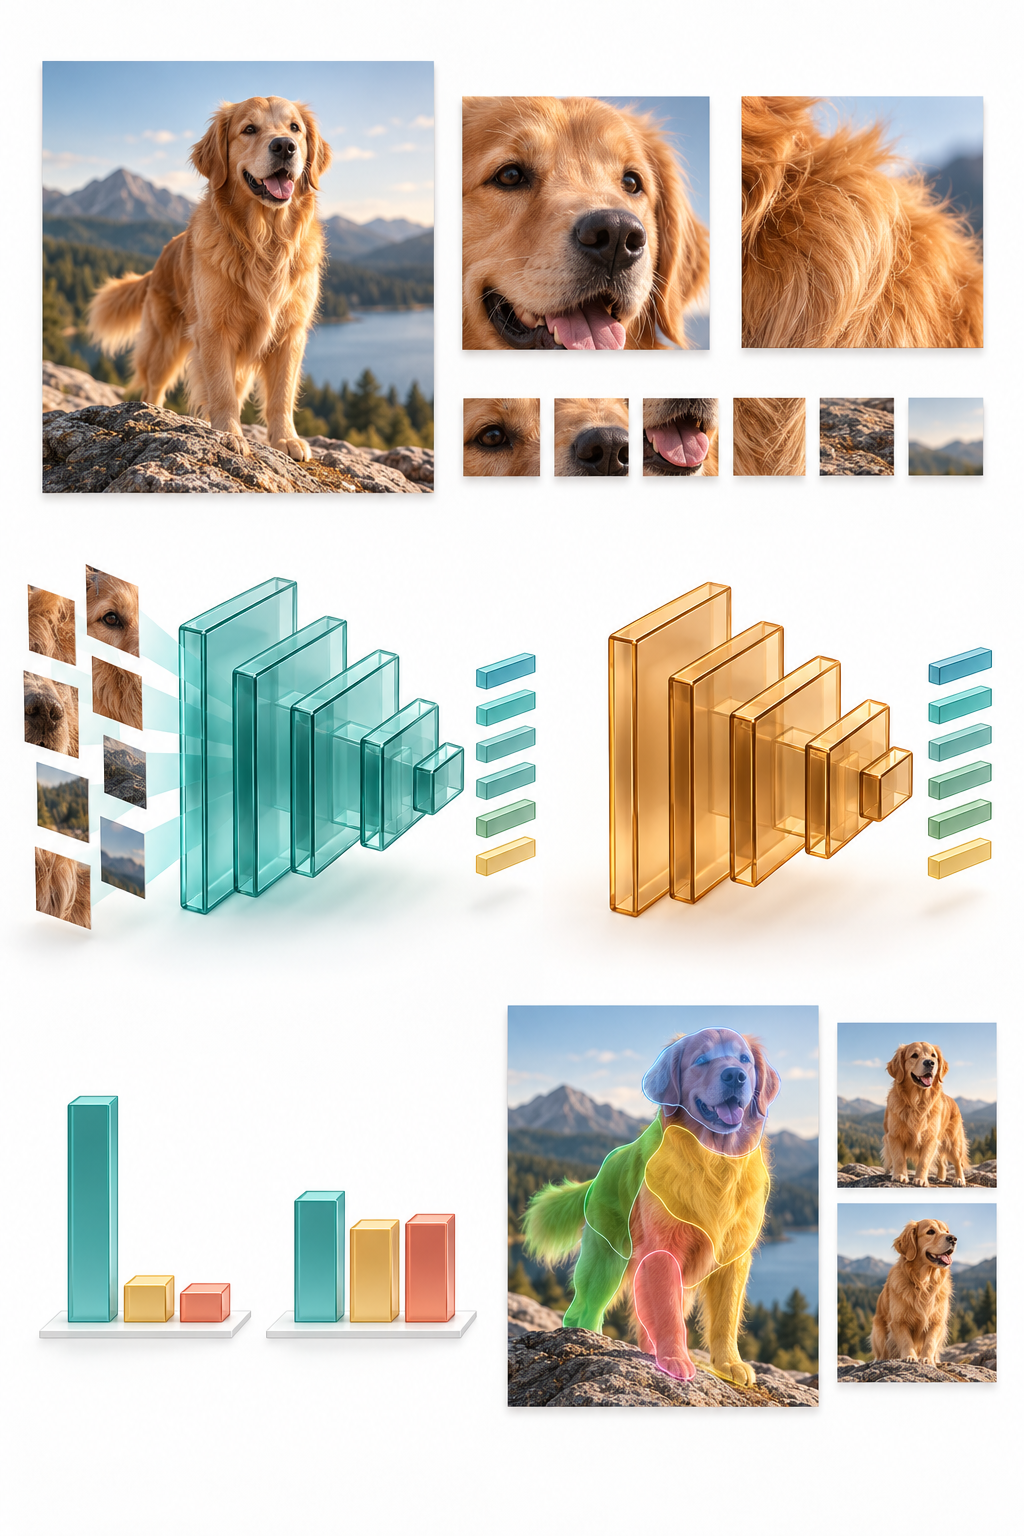
\includegraphics[width=26mm,height=31mm,keepaspectratio,viewport=20 46 520 506,clip]{dino-imagegen-draft.png}};
\draw[-{Latex[length=2mm]},teal,line width=.7pt] (52.5,98.5) -- (52.5,95);
\fill[warm,rounded corners=2mm] (1,53) rectangle (104,94);
\node[anchor=north west,text=teal,font=\bfseries\fontsize{12}{15}\selectfont] at (4,92) {D 教师慢慢跟上 · §3.1};
\node[anchor=north west,text width=66mm,inner sep=0] at (4,84) {教师参数取学生的滑动平均\\$\theta_t\leftarrow\lambda\theta_t+(1-\lambda)\theta_s$\\中心由教师原始输出更新\\不是外部训练好的老师};
\node[anchor=center,inner sep=0] at (88,70) {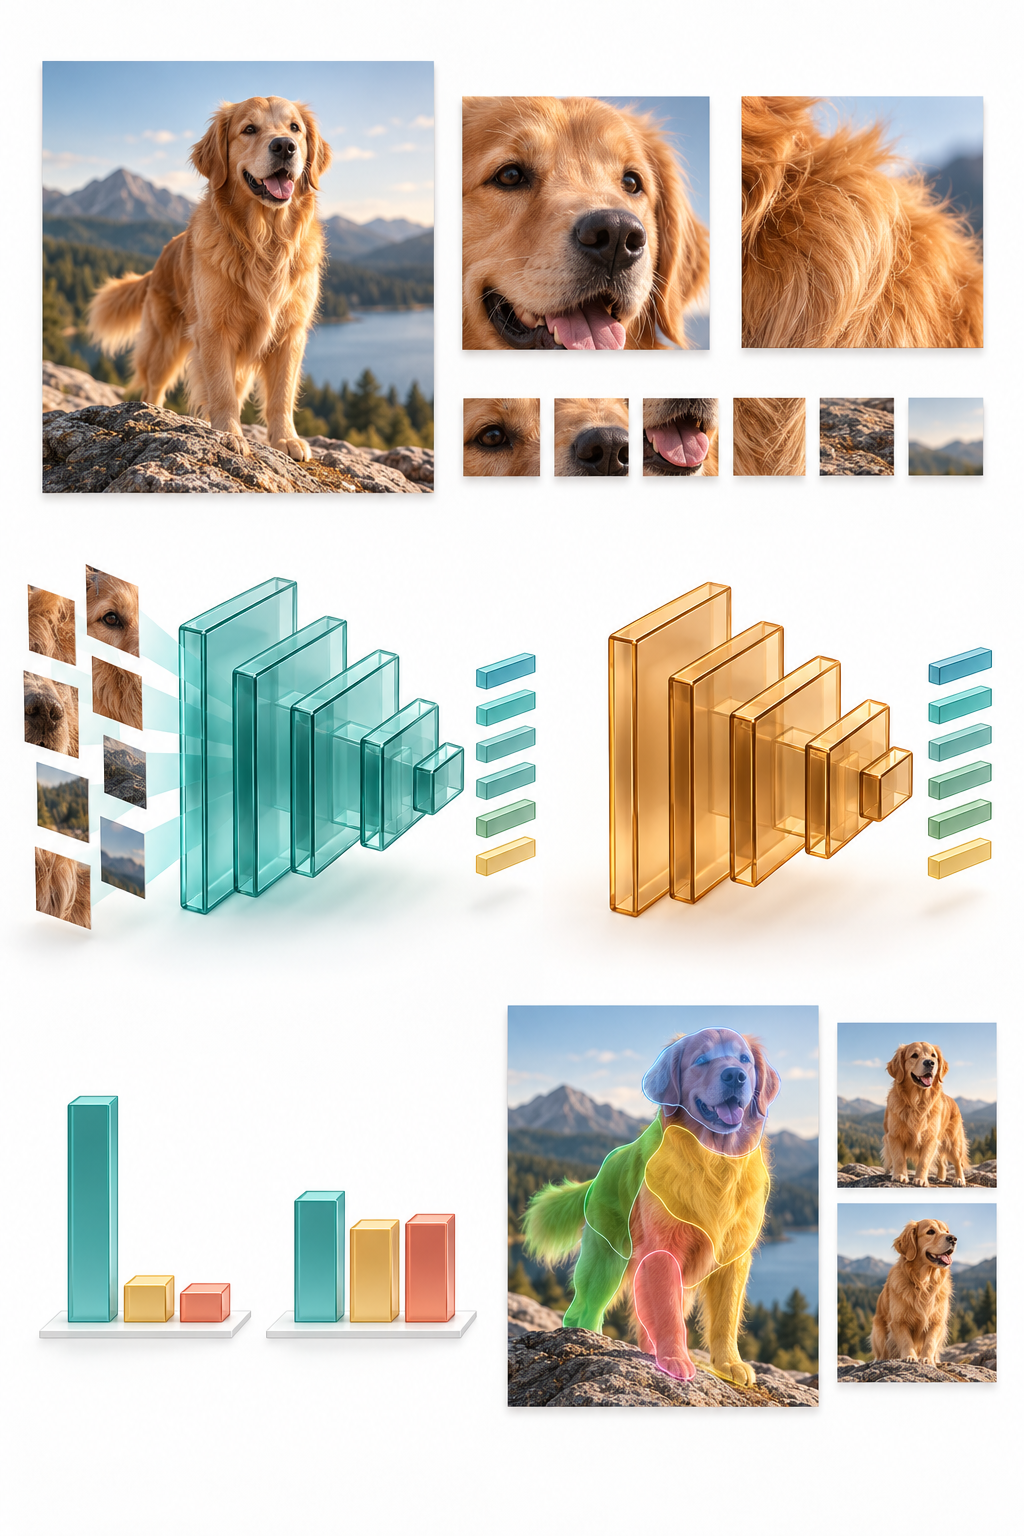
\includegraphics[width=26mm,height=31mm,keepaspectratio,viewport=530 536 1000 1046,clip]{dino-imagegen-draft.png}};
\draw[-{Latex[length=2mm]},teal,line width=.7pt] (52.5,52.5) -- (52.5,49);
\fill[pale,rounded corners=2mm] (1,7) rectangle (104,48);
\node[anchor=north west,text=teal,font=\bfseries\fontsize{12}{15}\selectfont] at (4,46) {E 拿走视觉表示 · §4–5};
\node[anchor=north west,text width=66mm,inner sep=0] at (4,38) {去掉训练投影头\\CLS：近邻检索 / 分类\\patch：空间对应\\注意力图：观察物体区域};
\node[anchor=center,inner sep=0] at (88,24) {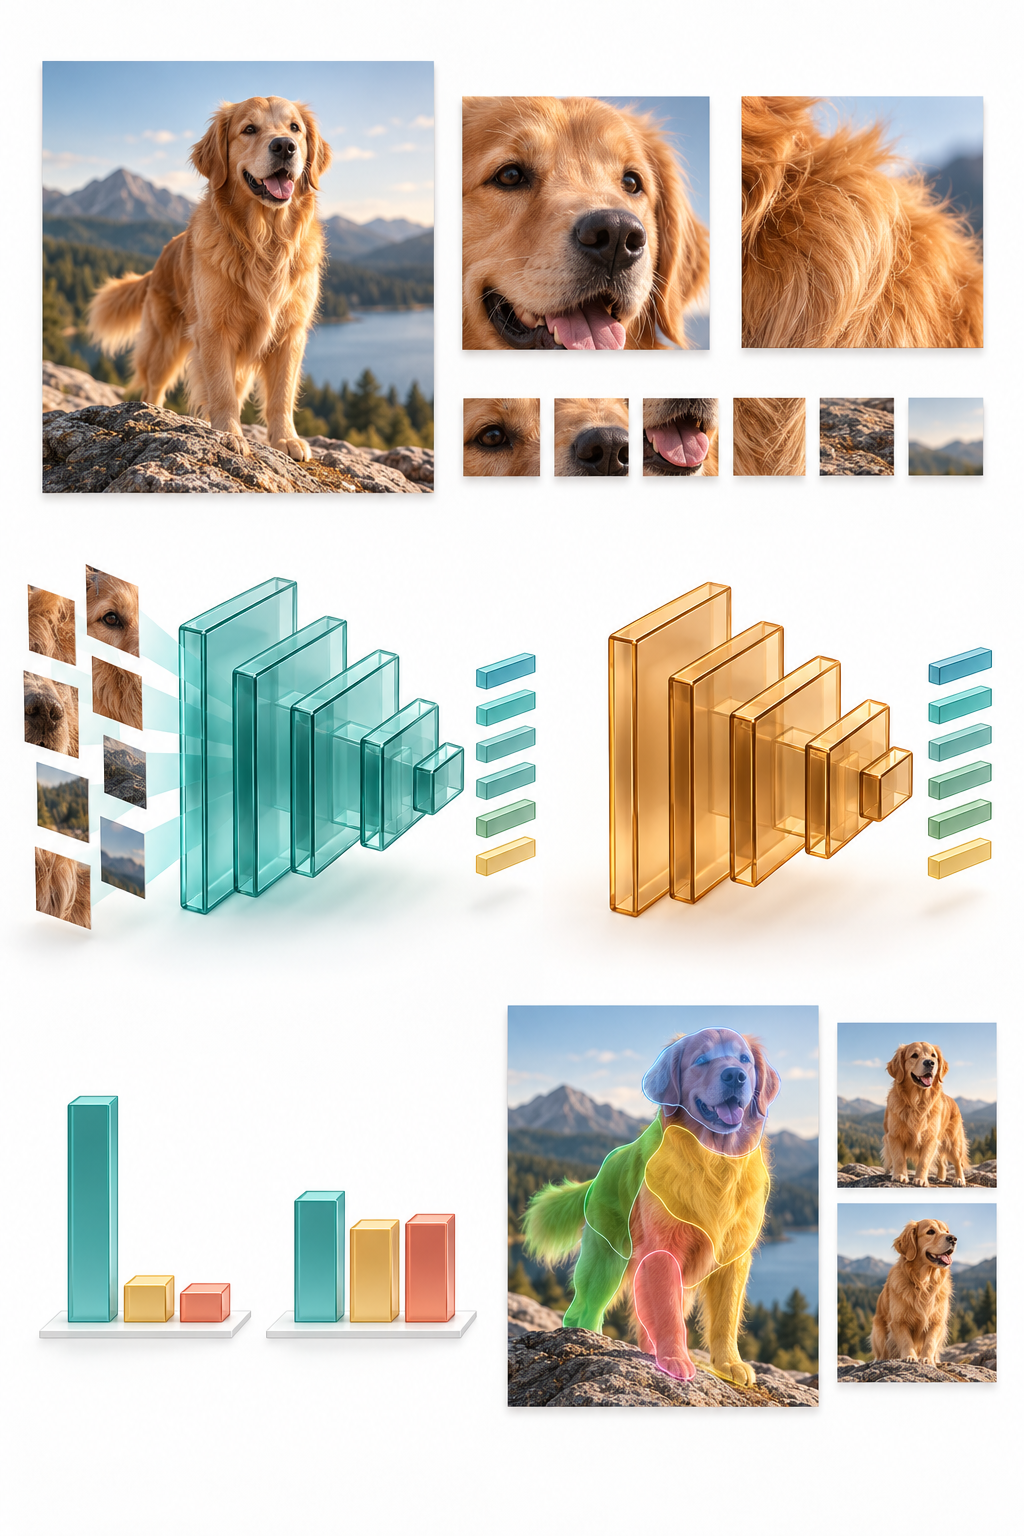
\includegraphics[width=26mm,height=31mm,keepaspectratio,viewport=520 26 1010 516,clip]{dino-imagegen-draft.png}};
\end{tikzpicture}\end{document}